\documentclass[11pt,a4paper,sans]{moderncv}  % Font sizes: 10, 11, or 12; paper sizes: a4paper, letterpaper, a5paper, legalpaper, executivepaper or landscape; font families: sans or roman
\moderncvstyle{classic}          % CV theme - options include: 'casual' (default), 'classic', 'oldstyle' and 'banking'
\moderncvcolor{orange}           % CV color - options include: 'blue' (default), 'orange', 'green', 'red', 'purple', 'grey' and 'black'
\usepackage[utf8]{inputenc}         % UTF8 para meter acentos y enies
\usepackage[scale=0.75]{geometry}      % Reduce document margins
%----------------------------------------------------------------------------------------
%  NAME AND CONTACT INFORMATION SECTION
%----------------------------------------------------------------------------------------
\firstname           { Pablo                                                               }
\familyname          { Slavkin                                                             }
\title               { Currículum Vitae                                                    }
\address             { Piedras 689, Bariloche                                              }{ Río Negro, Argentina }
\birth               { 13/12/1976                                                          }
\mobile              { (+54)(911) 6 243 3463                                               }
\phone               { (+54)(2944) 459 671                                                 }
\email               { pslavkin@disenioconingenio.com.ar                                    }
\homepage            { www.disenioconingenio.com.ar/categoria.php?css=1\&categories_id=191 }{ Online CV            }
\photo[130pt][0.4pt] {./pictures/cara2018.png}

%para generar links de una seccion a otra como no estan numeradas usar
%\hyperlink{joselito}{link caption}
%\hypertarget{joselito}{}

%----------------------------------------------------------------------------------------
\begin{document}
\makecvtitle % Print the CV title
%----------------------------------------------------------------------------------------
%  EDUCATION SECTION
%----------------------------------------------------------------------------------------
\section{Presentación}
Soy ingeniero electrónico, recibido recientemente de especialista en sistemas
embebidos y cursando una maestría en sistemas embebidos. Trabajo todos los días
codificando en C, diseñando sistemas embebidos de tiempo real desde bare metal
hasta FreeRTOS, desde la toma de requerimientos hasta la planificación, de los
test de aceptación de hard y soft, desde el esquemático y PCB hasta el
bootloader, desde el armado del prototipo a la documentación para la línea de
montaje.  Soy muy pragmático, disfruto resolver los problemas difíciles de modo
creativo e intercambiar mis ideas con mis pares. Soy extremadamente ordenado en
el desarrollo de firmware, PCB y en la administración de recursos.  Cuando no
estoy codificando, estoy tocando mal la guitarra, andando en bici o tomando una
caminata familiar.

\section{Educación}
\cventry { 2018--2018} { Especialización en sistemas embebidos} { FIUBA - Facultad de Ingeniería de Buenos Aires} { Buenos Aires}          { \textit { Promedio -- 9.33}}                                            { }
\cventry { 2007--2016} { Doctorado en Ingeniería}               { UTN - Universidad Tecnológica Nacional FRBA}    { Buenos Aires}          { \textit { Promedio -- 10 sobre 3 materias aprobadas + 3 finales adeudados}} { Mención Procesamiento digital de imágenes y señalesi. Suspendido por mudanza a otra ciudad}
\cventry { 1996--2005} { Ingeniería Electrónica}                { ITBA - Instituto Tecnológico de Buenos Aires}   { Buenos Aires}          { \textit { Promedio -- 6.5}}                                                 { }
\cventry { 1990--1995} { Técnico Electromecánico}               { ENET Nº1 Brigadier General Pascual Echagüe}     { Concordia, Entre Ríos} { \textit { Promedio -- 8.5}}                                                 { }
\cventry { 1982--1989} { Escuela Primaria}                      { Escuela Velez Sarsfield}                        { Concordia, Entre Ríos} { \textit { Promedio -- 8.5}}                                                 { }
%----------------------------------------------------------------------------------------
%  WORK EXPERIENCE SECTION
%----------------------------------------------------------------------------------------
\section{Experiencia}
   \subsection{Profesional}
      \cventry { 2005--Presente} { Director en empresa de ingeniería}                 { \href { www.disenioconingenio.com.ar} { disenioconingenio}} { } { } { Emprendimiento personal. Estudio de ingeniería que ofrece servicios de diseño electrónico a empresas, con capacidad para desarrollar y fabricar equipos electrónicos, hardware, firmware, software, mecánica, ruteo de PBC's, montaje de PCB's SMD y TH, impresión 3D, mecanizado CNC, corte y grabado laser y comercializa equipos para control de accesos RFID, monitoreo de temperatura ethernet, automatización de maquinas, conversores de protocolos, etc. \href { http://disenioconingenio.com.ar/producto.php?products_id=398} { ver detalles}}
      \cventry { 2011--2014}     { Consultor y desarrollador de equipos electrónicos} { \href { www.seconsat.com}             { Seconsat}}          { } { } { Consultoría y desarrollo de accesorios electrónicos para el rubro AVL. \hyperlink{subsec:seconsat}{ver portfolio}}
      \cventry { 2003--2005}     { Desarrollador de equipos electrónicos}             { \href { www.digicard.com.ar}          { Digicard}}          { } { } { Empresa referente a nivel nacional en el rubro de control de accesos. Se trabajo en el desarrollo de un lector RFID de 125khz para la linea de controladores de accesos. Se participo en todas las etapas desde el requerimiento, diseño, layout, prototipo, puesta en marcha, firmware, documentación general y para producción. Actualmente es un producto comercializado activamente por la empresa. \href                                                          { http://disenioconingenio.com.ar/producto.php?products_id=393} { ver detalles}}
      \cventry { 2002--2003}     { Desarrollador de firmware para microcontroladores} { \href { www.pump-control.com.ar}      { Pump-Control}}      { } { } { Empresa dedicada principalmente al diseño, desarrollo y producción de controladores electrónicos para la distribución de hidrocarburos. Se trabajó en el área de desarrollo de firmware para microcontroladores de 8bits de la linea Atmel, implementando protocolos de comunicaciones, control de accesos, control de dispenser de combustible, etc. \href                                                                                                            { http://disenioconingenio.com.ar/producto.php?products_id=391} { ver detalles}}

   \subsection{Investigación}
      \cventry { 2015--2016 }{ Becario en la Comisión Nacional de Energía Atómica                 }{ \href { https://www.cnea.gob.ar    }{ CNEA    } }{ }{ }{ Se trabaja como becario en la culminación de un PET (Positron Emission Tomography) íntegramente desarrollado en el centro sobre el cual se desarrolla el plan de tesis doctoral. Particularmente se trabaja en el área de adquisición y procesamiento de señales digitales sobre FPGA de alta performance. Se termina la beca por mudanza a otra ciudad \href { http://disenioconingenio.com.ar/producto.php?products_id=455 }{ ver material 2015 }, \href { http://disenioconingenio.com.ar/producto.php?products_id=456 }{ ver material 2016 } }
      \cventry { 2009--2009 }{ Ayudante en el Centro de investigaciones de Láseres y Aplicaciones }{ \href { http://www.citedef.gob.ar/ }{ CITEDEF } }{ }{ }{ Se trabajó como ayudante del Dr. Jorge Codnia y la Lic. Laura Azcárate en el armado de un condensador de flujo láser para la generación de isótopos, y los primeros avances en un nuevo espectrómetro de masas de tiempo de vuelo                                                                                                                                                                                            }

   \subsection{Docencia}
      \cventry { 2017--2017} { Jornada de introducción a la robótica}                               { Siglo XXI} { } { } { Se dicto una jornada de introducción a la robótica para alumnos de tercer a quinto año}                     { }
      \cventry { 2004--2004} { Curso intensivo de programación de FPGA de Altera usando Quartus II} { ITBA}      { } { } { Se realizó un curso introductorio con actividades practicas usando una placa de evaluación de Altera. \href { http://disenioconingenio.com.ar/shop/docs/fpga.pdf} { ver material}}

   %\subsection{Otros Trabajos}
   %\cventry{1994--2001}{Instalación y mantenimiento de instalaciones eléctricas comerciales}   {}       {}{}{Se realizaron trabajos de electricidad, instalaciones eléctricas comerciales, reparaciones y mantenimiento general a clientes particulares}

\section{Cursos y seminarios}

\cventry [-0.5cm] { 2017 }{ LASCAS 2017 Tutorials: Dependable Digital Systems and Fault Tolerant FPGA Design }{ INVAP                                     }{ 8hs                                                                                                                                 }{                                                                                                                                                                }{                 }{ }
\cventry [-0.5cm] { 2017 }{ SASE 2017, Simposio Argentino de Sistemas Embebidos                              }{ UBA                                       }{ 8hs                                                                                                                                 }{ \href                                                                                           { http://disenioconingenio.com.ar/producto.php?products_id=444 }{ ver certificado }  }{ }{ }
\cventry [-0.5cm] { 2016 }{ SASE 2016, Simposio Argentino de Sistemas Embebidos                              }{ UBA                                       }{ 8hs                                                                                                                                 }{ \href                                                                                           { http://disenioconingenio.com.ar/producto.php?products_id=443 }{ ver certificado }  }{ }{ }
\cventry [-0.5cm] { 2015 }{ Encuentro Doctorado PSI – GIBIO – Modelos, Simulación e Ingeniería de Tejidos    }{ Favaloro                                  }{ 8hs                                                                                                                                 }{ \href                                                                                           { http://disenioconingenio.com.ar/producto.php?products_id=419 }{ ver certificado }  }{ }{ }
\cventry [-0.5cm] { 2015 }{ SASE 2015, Simposio Argentino de Sistemas Embebidos                              }{ UBA                                       }{ 6hs                                                                                                                                 }{ \href                                                                                           { http://disenioconingenio.com.ar/producto.php?products_id=411 }{ ver certificado }  }{ }{ }
\cventry [-0.5cm] { 2015 }{ Técnicas avanzadas de diseño digital                                             }{ UNICEN                                    }{ 40hs                                                                                                                                }{ Curso virtual avanzado de técnicas de diseño digital a cargo del ingeniero Guillermo Jaquenod                                                                  }{                 }{ }
\cventry [-0.5cm] { 2013 }{ SASE 2013, Simposio Argentino de Sistemas Embebidos                              }{ UBA                                       }{ 18hs                                                                                                                                }{                                                                                                                                                                }{                 }{ }
\cventry [-0.5cm] { 2012 }{ Primeras jornadas de procesamiento de señales e imágenes                         }{ UTN, GIBIO EDE2008 Electronic Design Expo }{ 8hs                                                                                                                                 }{ \href                                                                                           { http://disenioconingenio.com.ar/producto.php?products_id=396 }{ ver certificado }  }{ }{ }
\cventry [-0.5cm] { 2012 }{ SASE 2012, Simposio Argentino de Sistemas Embebidos                              }{ UBA                                       }{ 18hs                                                                                                                                }{                                                                                                                                                                }{                 }{ }
\cventry [-0.5cm] { 2011 }{ SASE 2011, Simposio Argentino de Sistemas Embebidos                              }{ UBA                                       }{ 18hs                                                                                                                                }{                                                                                                                                                                }{                 }{ }
\cventry [-0.5cm] { 2010 }{ SASE 2010, Simposio Argentino de Sistemas Embebidos                              }{ UBA                                       }{ 18hs                                                                                                                                }{                                                                                                                                                                }{                 }{ }
\cventry [-0.5cm] { 2008 }{ Conferencia sobre tecnologías inalámbricas de Digi RF                            }{ EDE2008 Electronic Design Expo            }{ 6hs                                                                                                                                 }{ \href                                                                                           { http://disenioconingenio.com.ar/producto.php?products_id=394 }{ ver certificado }  }{ }{ }
\cventry [-0.5cm] { 2007 }{ Curso teórico práctico de serigrafía orientado a la fabricación de PCB's         }{ 32hs                                      }{ \href                                                                { http://disenioconingenio.com.ar/producto.php?products_id=389 }{ ver detalles                                                                                                                                                   }                  }{ }{ }
\cventry [-0.5cm] { 2007 }{ Seminario de desempeño analógico usando microcontroladores Silabs                }{ 8hs                                       }{ \href                                                                { http://disenioconingenio.com.ar/producto.php?products_id=395 }{ ver detalles                                                                                                                                                   }                  }{ }{ }
\cventry [-0.5cm] { 2006 }{ Lanzamiento microcontroladores Freescale RS08KA, acelerómetros y sensores        }{ 8hs                                       }{ \href                                                                { http://disenioconingenio.com.ar/producto.php?products_id=384 }{ ver certificado                                                                                                                                                }                  }{ }{ }
\cventry [-0.5cm] { 2006 }{ Lanzamiento microcontroladores Freescale Coldfire 32 bits                        }{ 10hs                                      }{ \href                                                                { http://disenioconingenio.com.ar/producto.php?products_id=385 }{ ver detalles                                                                                                                                                   }                  }{ }{ }
\cventry [-0.5cm] { 2004 }{ Microprocesadores Rabbit y Dinamic C                                             }{ 24hs                                      }{ \href                                                                { http://disenioconingenio.com.ar/producto.php?products_id=386 }{ ver certificado                                                                                                                                                }                  }{ }{ }
\cventry [-0.5cm] { 2002 }{ Curso teórico práctico IA “Inteligencia Artificial”                              }{ ITBA                                      }{ 18hs                                                                                                                                }{ \href                                                                                           { http://disenioconingenio.com.ar/producto.php?products_id=387 }{ ver certificado }  }{ }{ }
\cventry [-0.5cm] { 1995 }{ Curso de radio aficionado con obtención de licencia LU9JGM                       }{ Radio Club Concordia (LU9JJ)              }{ 48hs                                                                                                                                }{ \href                                                                                           { http://disenioconingenio.com.ar/producto.php?products_id=388 }{ ver detalles    }  }{ }{ }
%----------------------------------------------------------------------------------------
%  AWARDS SECTION
%----------------------------------------------------------------------------------------
\section{Premios}
\cventry{2002 }{Iniciación en I+D ITBA                                 }{1\textsuperscript{er }Premio }{ }{ }{\em{Diseño y Simulación de una Unidad de Punto Flotante con estructura Pipeline Multi-Thread para procesadores de propósitos generales de alta performance }\em \href{http://disenioconingenio.com.ar/shop/docs/i+d_itba_2002.pdf                                                                                                                                                                       }{ver mas } }
\cventry{2001 }{Robots de lucha Battle Tek, ITBA ``ingenio en acción'' }{3\textsuperscript{er }Puesto }{ }{ }{\em{Robot Discotech                                                                                                                                        }\newline \em{Se diseño y fabricó un robot de lucha basado en un disco giratorio de alta velocidad de rotación con 2 salientes filosas que impactan contra el adversario. \href{http://disenioconingenio.com.ar/producto.php?products_id=378 }{ver mas } } }
%----------------------------------------------------------------------------------------
%  COMPUTER SKILLS SECTION
%----------------------------------------------------------------------------------------
\section{Trabajos y publicaciones}
\cventry { 2018 }{ Controlador para máquina CNC de 3 ejes                                                                                                      }{ Especialización en sistemas embebidos, FIUBA                  }{                                                            }{ }{ Trabajo final de la carrera de especialización en sistemas embebidos, Director: Ing. Juan Manuel Cruz \href                             { http://                                                     }{ ver trabajo                                                                                                            }                                                                                                          }
\cventry { 2010 }{ Suavizado de imágenes por difusión inhomogénea                                                                                              }{ Procesamiento de imágenes Biomédicas, UTN                     }{                                                            }{ }{ Trabajo final Procesamiento de imágenes biomédicas, Tutor: Dr. Castro \href                                                             { http://disenioconingenio.com.ar/shop/docs/Final_ooffice.pdf }{ ver trabajo                                                                                                            }                                                                                                          }
\cventry { 2008 }{ Estudio de técnicas foto térmicas aplicadas a la medición de flujo gaseoso                                                                  }{ CITEDEF                                                       }{                                                            }{ }{ Se presentó bajo la tutela Dr. Francisco Manzano y como meta de aprobación de Optoelectrónica II. \href                                 { http://disenioconingenio.com.ar/shop/docs/citedef_2008.pdf  }{ ver trabajo                                                                                                            }                                                                                                          }
\cventry { 2004 }{ Diseño e implementación de una pantalla dinámica basada en 3200 lámparas de filamento con 16 escalas de grises y 20fps actualizable por ftp }{ LampMatrix, Tesis de grado, ITBA                              }{                                                            }{ }{ Bajo la tutela del Profesor Villamil, se diseñó y fabricó íntegramente una pantalla publicitaria basada en lamparas de filamento. \href { http://www.youtube.com/watch?v=Usx4YUNpknc                  }{ ver video                                                                                                              }, \href                                        { http://disenioconingenio.com.ar/shop/docs/lampmatrix.pdf }{ ver trabajo }. }
\cventry { 2003 }{ Design and Simulation of a pipeline-structured Floating Point Unit for high performance general purpose processors                          }{ JAIIO 32\textsuperscript                                 { as }Jornadas Argentinas de Informática e Investigación Operativa }{ }{                                                                                                                                                                                                       }{ \href                                                        { http://disenioconingenio.com.ar/shop/docs/jaiio2003.pdf }{ ver trabajo                                                                                             }              }
\cventry { 2003 }{ Selección del número de etapas óptimas en unidades de punto flotante con estructura pipeline                                                }{ CACIC, Congreso argentino de ciencias de la computación       }{                                                            }{ }{ \href                                                                                                                                   { http://disenioconingenio.com.ar/shop/docs/cacic2003.pdf     }{ ver trabajo                                                                                                            }                                                                                                          }
%----------------------------------------------------------------------------------------
\section{Dominio de tecnologías}
   \subsection{Sistamas Operativos}
      \cvitem { Avanzado}   { Linux (Debian, Crunchbang, Bunsenlabs, Ubuntu), FreeRTOS, Windows(XP, Seven, Server2003, Office2000) }
      \cvitem { Intermedio} { FreeBSD}
      \cvitem { Básico}     { OSEK}

   \subsection{Programas de computadora destacados}
      \cvitem { Avanzado   }{ crypsetup, vim, mutt, git, mercurial, gnumeric, ssh, bash, screen, tmux, pass, Allegro PCB Router, Slic3r, Pronterface, Mach3, LinuxCNC, Rhinoceros, RhinoCam, Orcad16 ( Design CIS,Layout,Pspice ),  Flash MX, Borland C++ Builder, Octave, Wireshark, gcc, Xilinx (ISE y Vivado), Microsoft Visual Studio, VirtualBox, gdb, openocd, redmine, cups, Swat, Samba, Cura, Freecad, ceedling , gnuplot, ncurses, cdk, Kicad, \LaTeX}
      \cvitem { Intermedio }{ OpenOffice, LibreOffice, Matlab, Mathcad, quemu, Arduino, svn, ffmpeg, Openscam, Webadmin, SonarQube }
      \cvitem { Básico     }{ Quartus II, Delphi, Eclipse, Blender }

   \subsection{Lenguajes de programación}
      \cvitem { Avanzado}   { C, Octave, Verilog, assembler, VHDL}
      \cvitem { Intermedio} { C++, C\#,  Pascal, bash, makefiles, openHab, Microsoft Visual Studio}
      \cvitem { Básico}     { Java, Javascript, \textsc { html}, Python}

   \subsection{Microcontroladores, microprocesadores y FPGA}
      \cvitem { Avanzado   }{ Freescale(HC9S08 8b (JM, MC13x, MP, GT, SH, SE, QD, AC, QE) , HC11 8b, HCS12 16b (NE64, C), Coldfire V2 32b (MCF51JMx, MCF522x), Kinetis ARM Cortex-M0 32b(E,W), Kinetis ARM Cortex-M4 32b(K,KE)), NXP(LPC54628), Atmel AtmegaXX 8b, Texas ARM Cortex-M4 32b(CC3200, TM4C129x), Xilinx (Spartan3, Spartan6, Arty7) }
      \cvitem { Intermedio }{ Rabbit 2200 8b, Altera Flex 10K10, Microchip Pic168xa                                                                                                                                                                                                                                                              }
      \cvitem { Básico     }{ Texas MSP430 16b, Scilabs 8b                                                                                                                                                                                                                                                                                       }

   \subsection{Protocolos de comunicaciones y técnicas digitales}
      \cvitem{Avanzado   }{TCP, IPv4, SNMP, SMTP, NTP, ARP, Ethernet, UDP, SCI, SPI, I2C, LVDS, USB FS/HS, Zigbee, RFID, PWM, ADC, DAC, 1-Wire, RS232, RS485, PoE+ }
      \cvitem{Intermedio }{IPv6, CAN, 6LoWPAN, IEEE 802.15.4, lwIP, I2S, Radius, Modbus                                                                            }
      \cvitem{Básico     }{                                                                                                                                        }

   \subsection{Otras tecnologías de Interés}
      \cvitem{Avanzado   }{Manejo de línea de montaje SMD, Soldado de PCB's manual por horno y ola, Impresión 3D FDM, serigrafía sobre rigido, serigrafía de PCB's,  mecanizado CNC, Manejo de maquina de corte laser, manejo de máquinas herramientas }
      \cvitem{Intermedio }{Manufactura de PCB's                                                                                                                                                                                                        }
      \cvitem{Básico     }{                                                                                                                                                                                                                            }
%----------------------------------------------------------------------------------------
%  LANGUAGES SECTION
%----------------------------------------------------------------------------------------
\section{Idiomas}
\cvitemwithcomment { Español }{ Oral/Lectura/Escritura Avanzado           }{ Lengua nativa                                                                        }
\cvitemwithcomment { Inglés  }{ Oral/Lectura/Escritura Intermedio         }{ TOEIC 2005--785 \href { http://disenioconingenio.com.ar/producto.php?products_id=390 }{ ver certificado } }
\cvitemwithcomment { Hebreo  }{ Lectura Intermedio, Escritura/Oral Básico }{ Escuela primaria hebrea completa                                                     }

\selectlanguage{spanish}
\section{Portfolio}
   \subsection{Seconsat}
   \hypertarget{subsec:seconsat}
   Ademas de las tareas de consultoría, se desarrolló un equipo inalámbrico para reporte de temperatura, humedad, velocidad, y demás parámetros desde la caja de un camión de carga a un equipo rastreador. \\
   Se utilizó tecnología 0402 en una placa de 4 capas con requerimientos de radiofrecuencia desde 200 Mhz hasta 2.4 Ghz. \\
   Se definieron los requerimientos, se diseñó el esquematico, y se diseñó el PCB en Orcad Allegro como se muestra en la figura \ref{fig:seconsat1}.
   \begin{figure}
      \begin{center}
         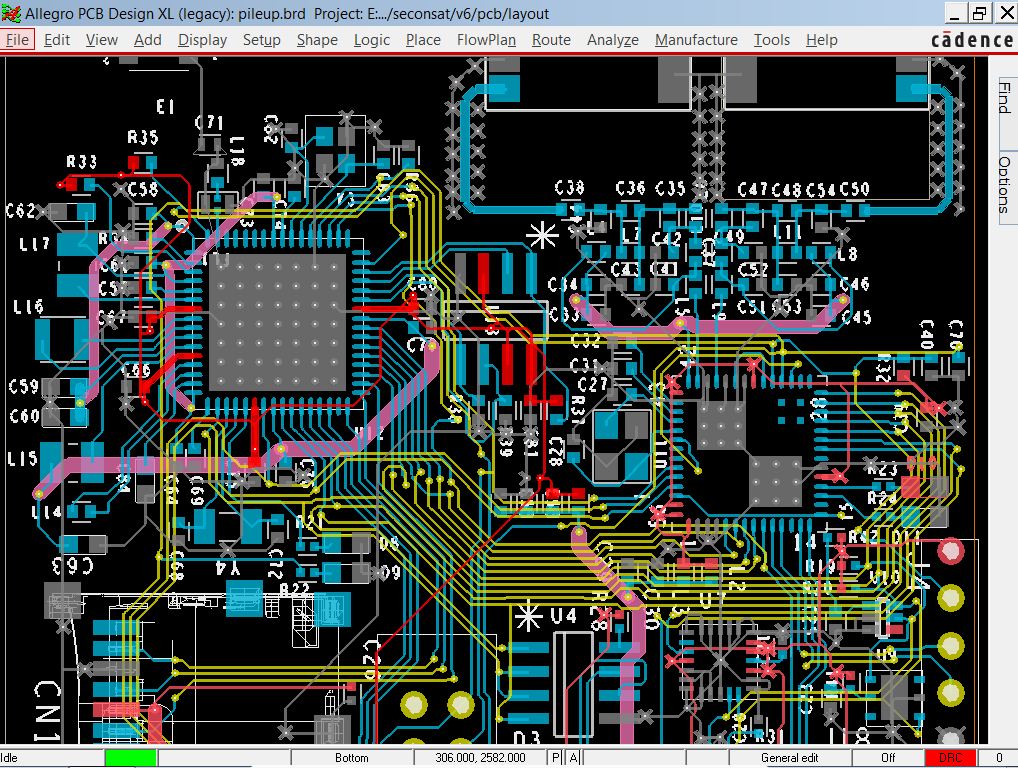
\includegraphics[width=0.49\textwidth]{./portfolio/seconsat1.png}
         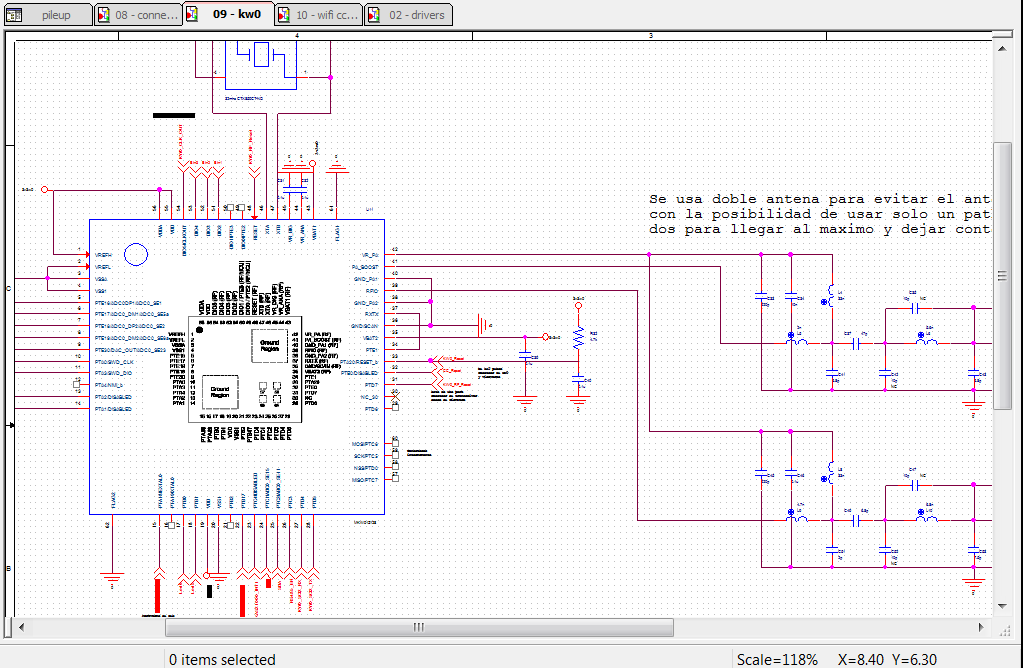
\includegraphics[width=0.49\textwidth]{./portfolio/seconsat2.png}
      \end{center}
      \caption{Desarrollo de PCB de comunicación inalámbrica 2.4Ghz y sub-1Ghz para reporte de parámetros ambientales dentro de camiones}
      \label{fig:seconsat1}
   \end{figure}

   \subsection{Noto Group S.A.}
   \hypertarget{subsec:noto}
   Para la empresa Noto Group S.A se desarrollan y se fabrican actualmente
   equipos electrónicos para electromedicina estética entre los que se destacan:
   \begin{itemize}
      \item{Radiofrecuencia tripolar.}
      \item{Electroporador.}
      \item{Microdermoabrasión.}
      \item{Cavitador.}
      \item{Luminoterapia.}
      \item{Electroestimulador portátil.}
      \item{Fuentes de alimentación categoría medica.} \\
   \end{itemize}
   En la figuras \ref{fig:noto1} y \ref{fig:noto2} se muestran algunos de los equipos desarrollados y fabricados:
   \begin{figure}
      \begin{center}
         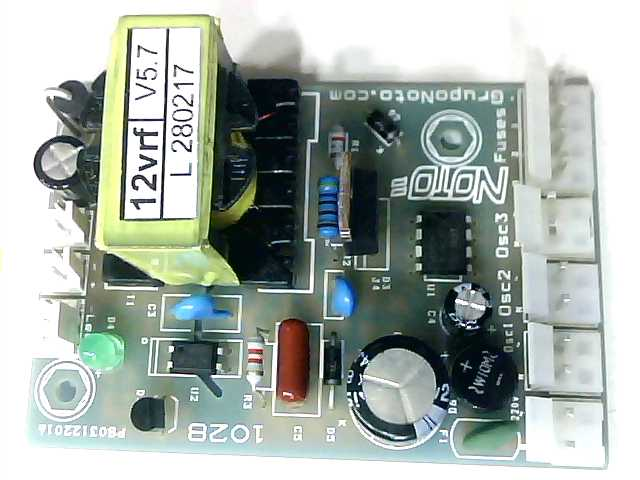
\includegraphics[width=0.49\textwidth]{./portfolio/fuente.jpg}
         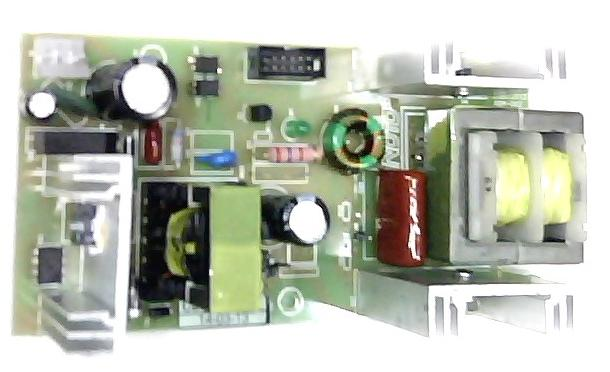
\includegraphics[width=0.49\textwidth]{./portfolio/cavi.jpeg}
         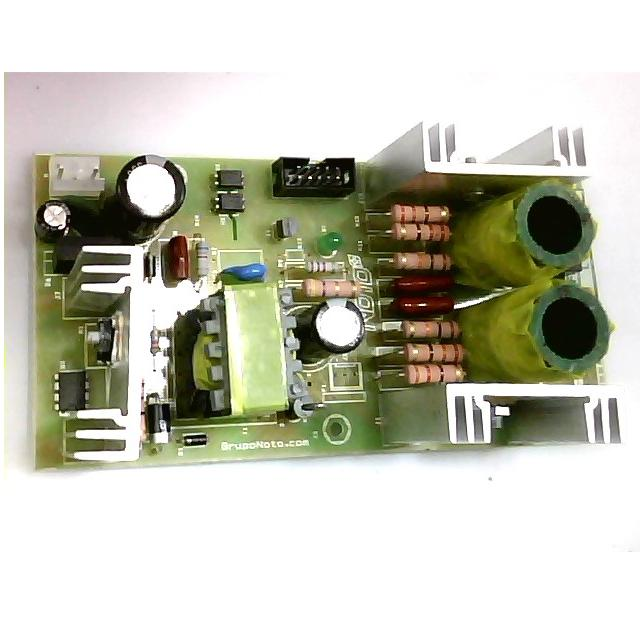
\includegraphics[width=0.49\textwidth]{./portfolio/trimax.jpeg}
         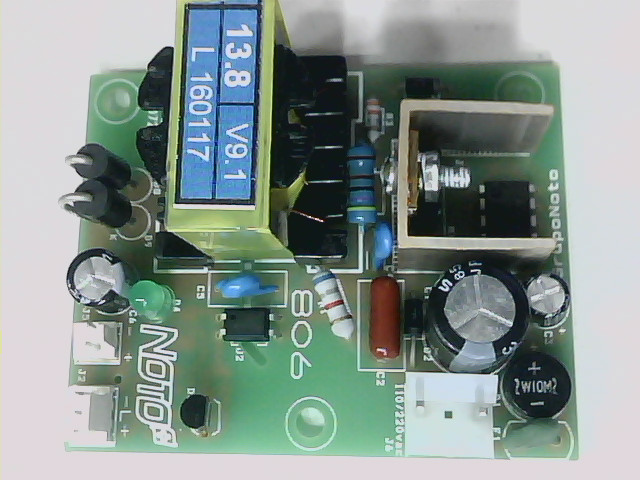
\includegraphics[width=0.49\textwidth]{./portfolio/fuente_13.jpeg}
      \end{center}
      \caption{Equipos de potencia, fuentes, osciladores, mezclando tecnologias TH y SMD}
      \label{fig:noto1}
   \end{figure}
   \begin{figure}
      \begin{center}
         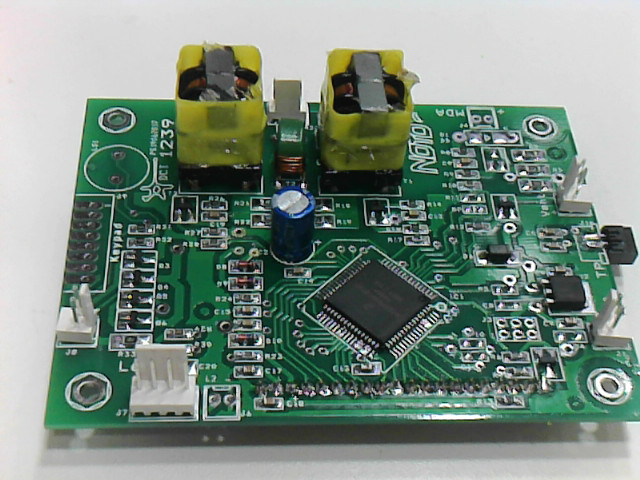
\includegraphics[width=0.49\textwidth]{./portfolio/n1500.png}
         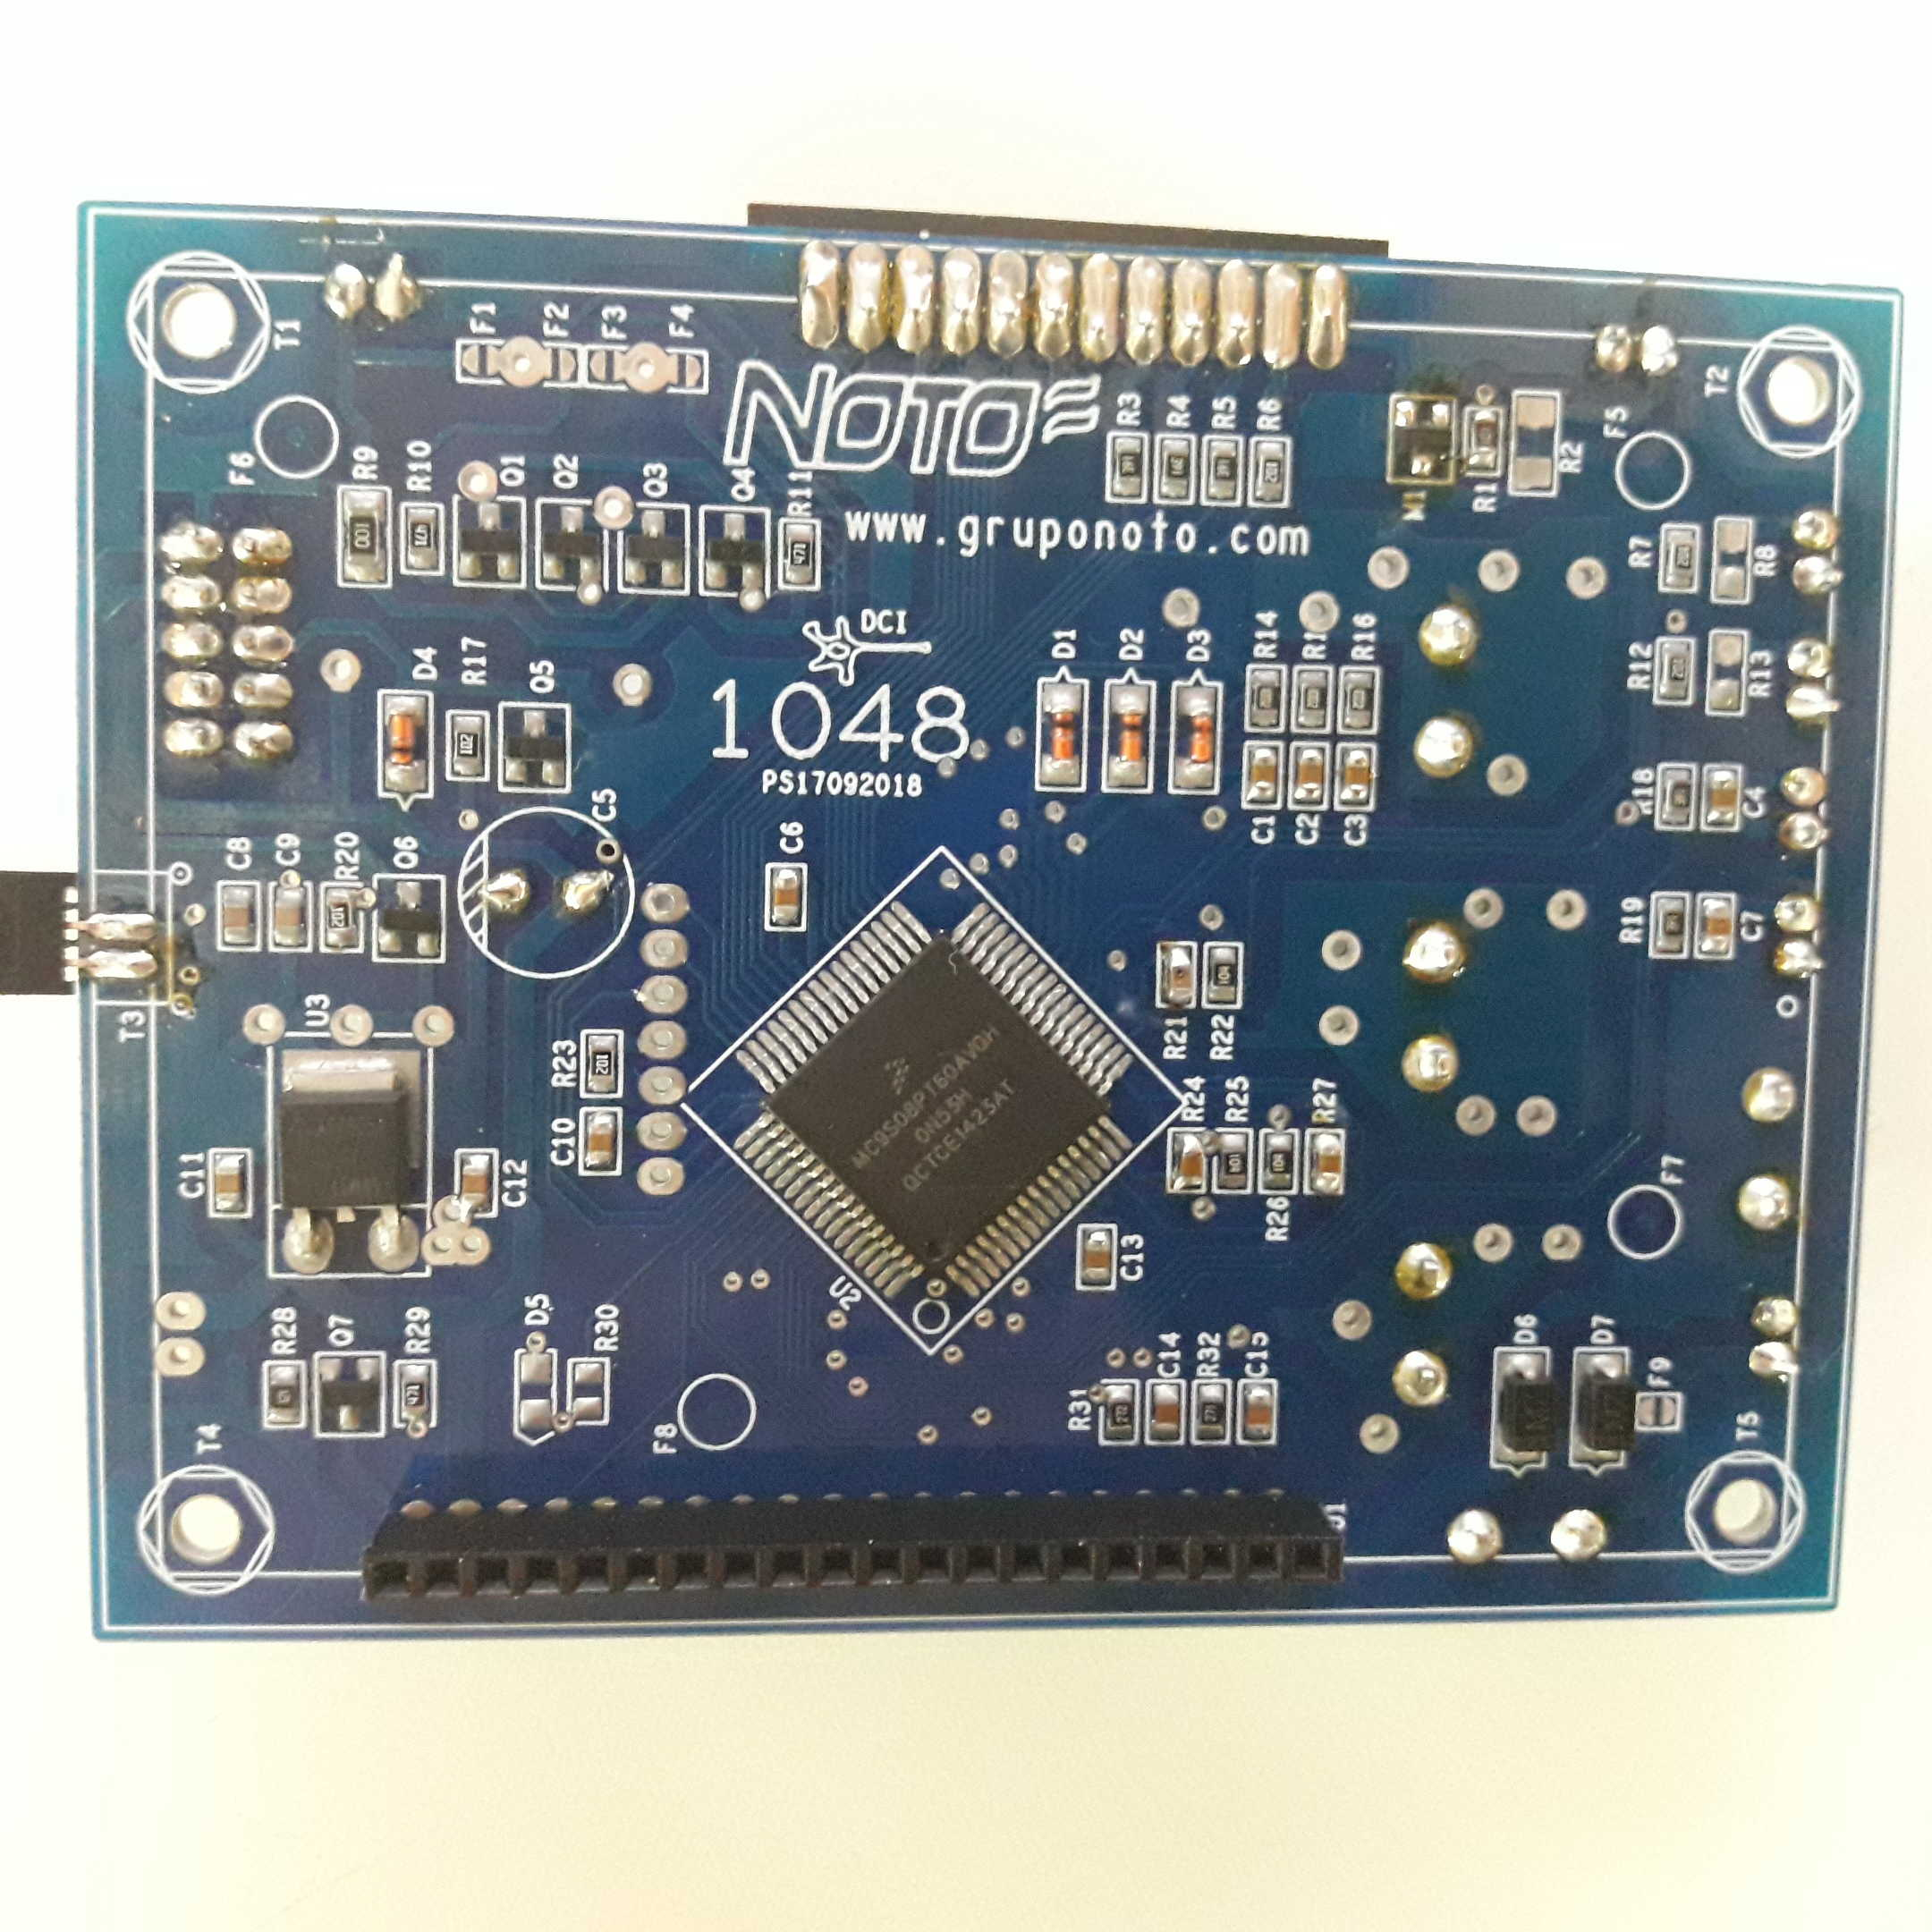
\includegraphics[width=0.49\textwidth]{./portfolio/lumiere.jpeg}
         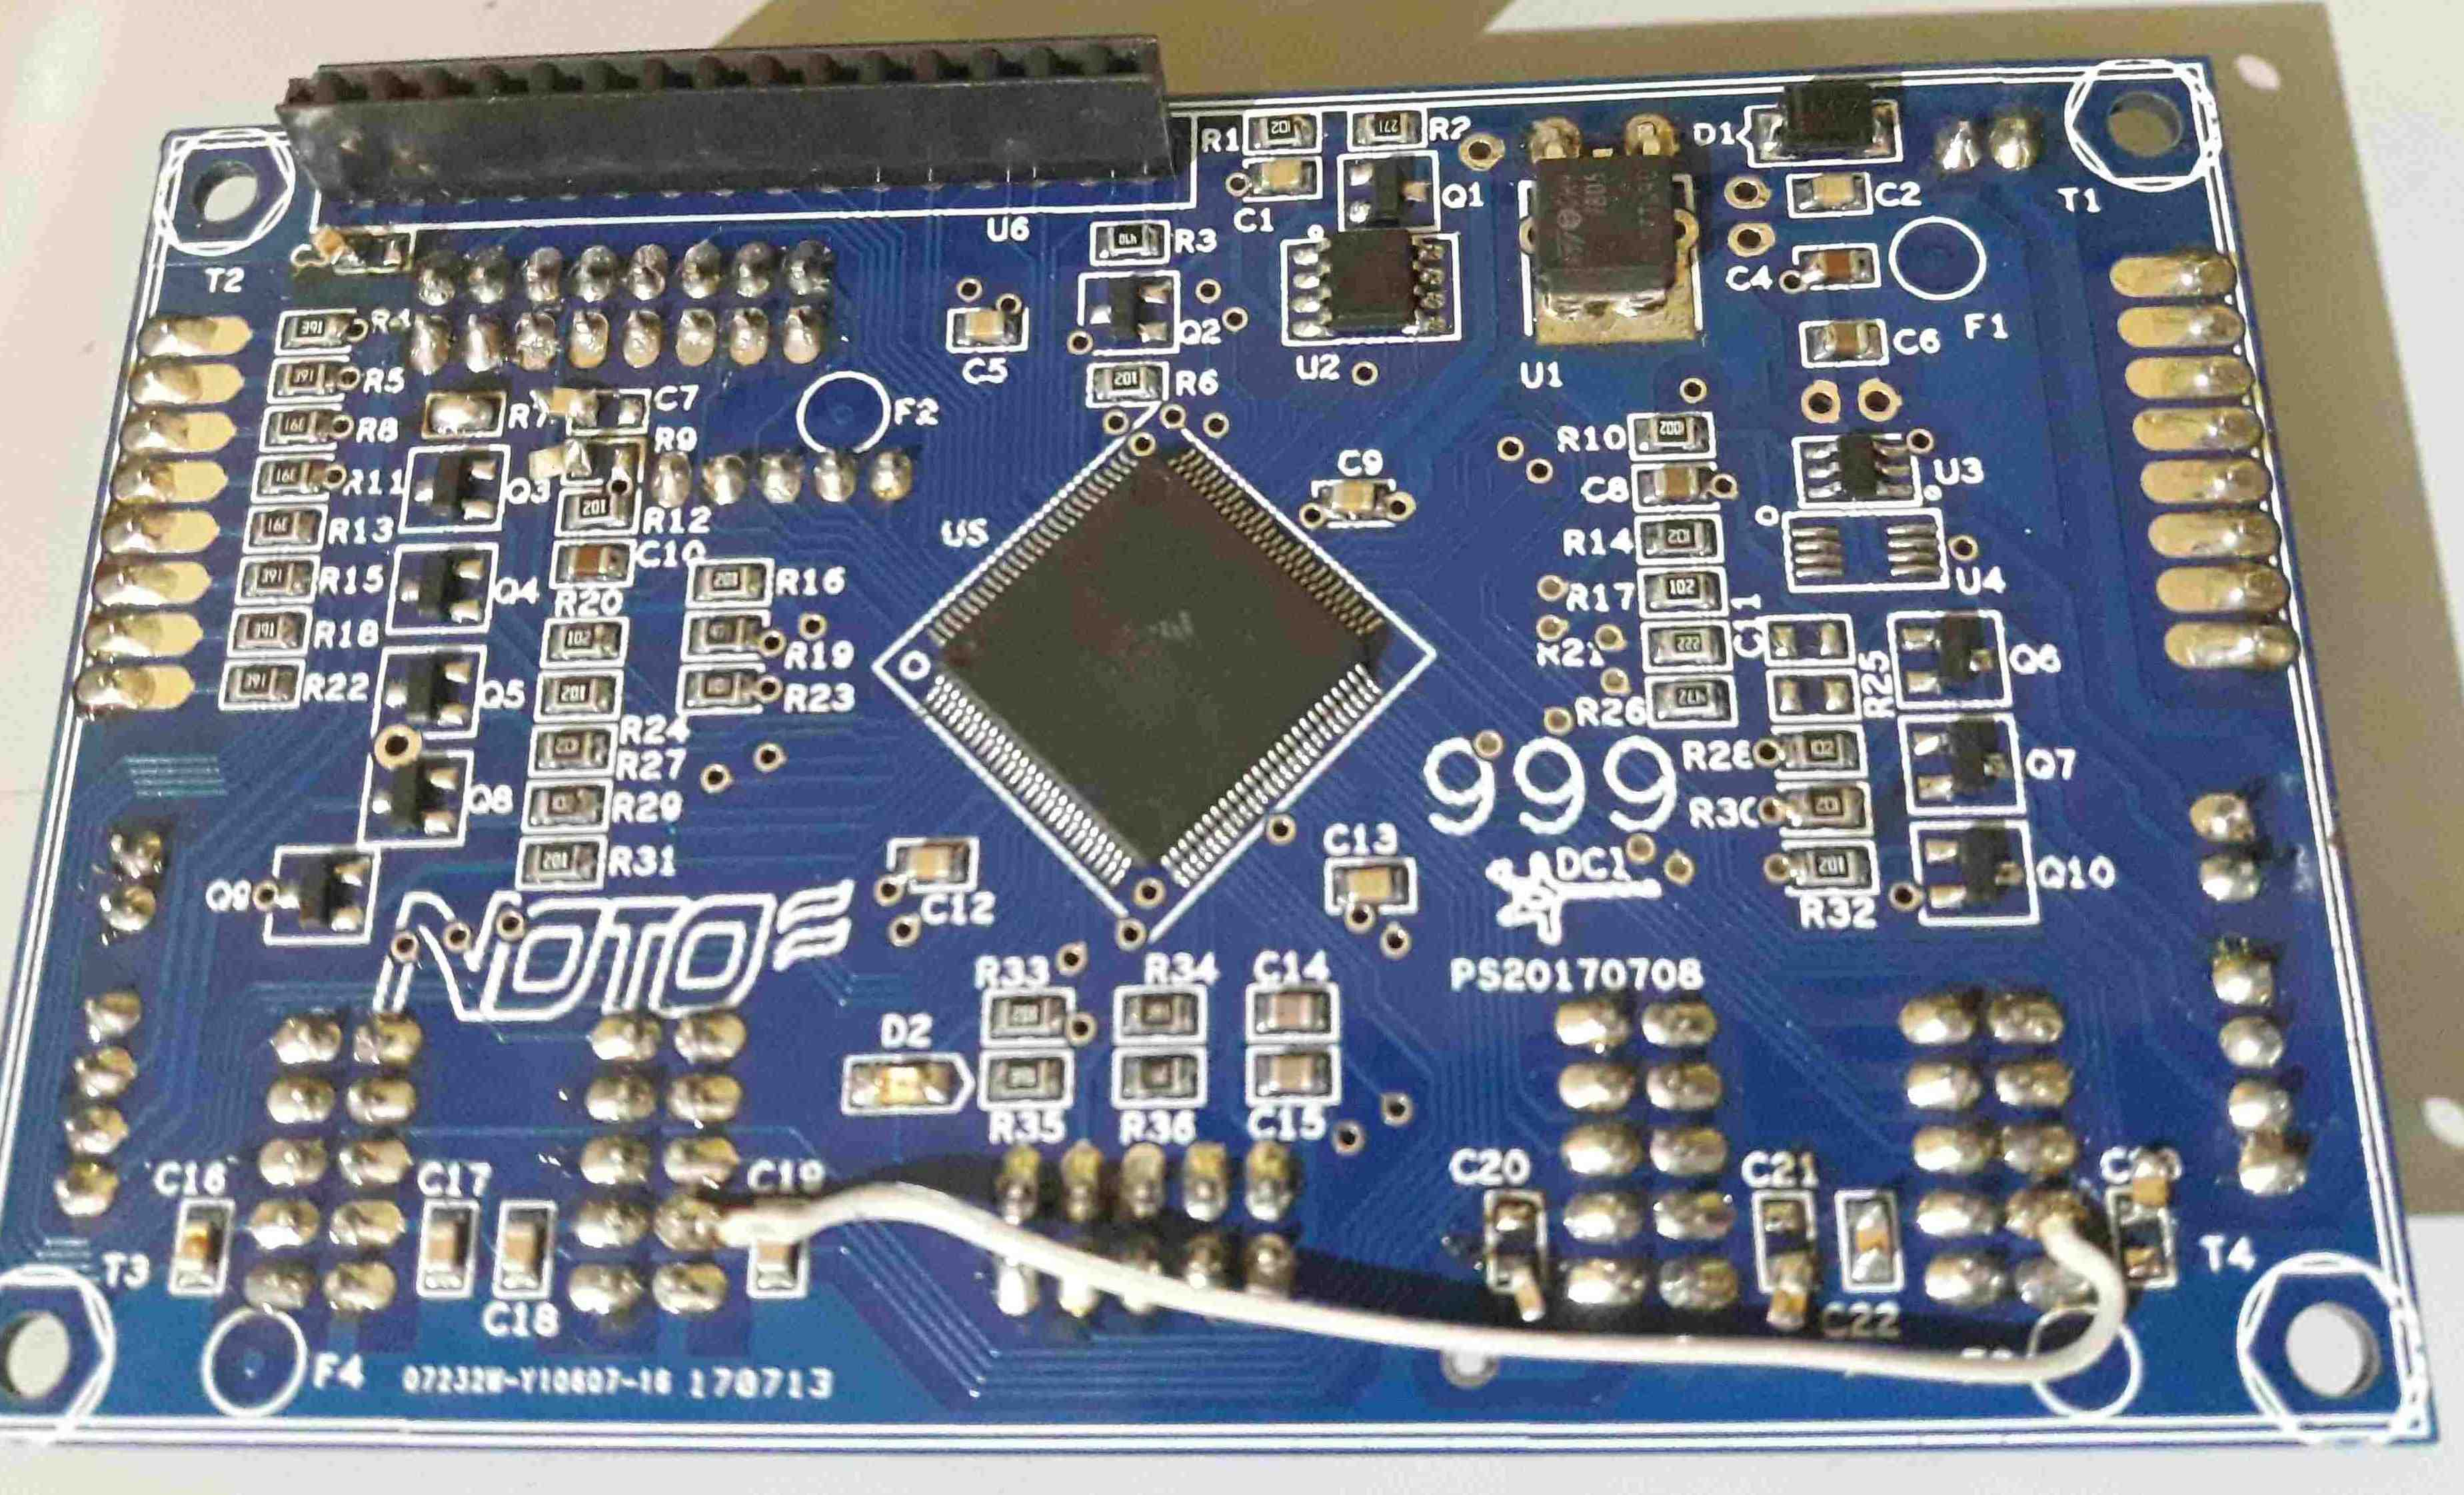
\includegraphics[width=0.49\textwidth]{./portfolio/electroestimulador.jpg}
         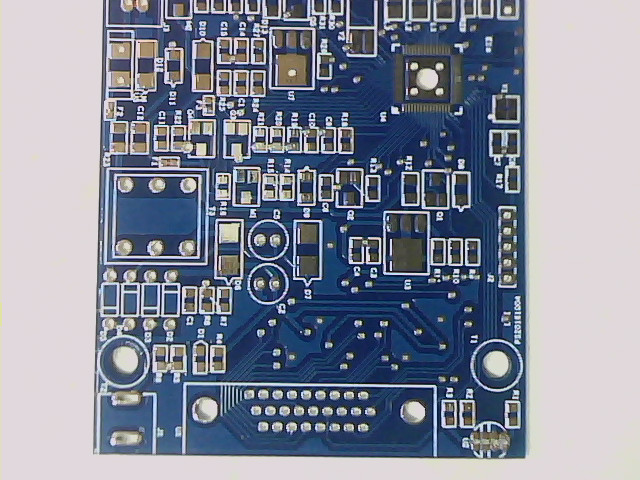
\includegraphics[width=0.49\textwidth]{./portfolio/electro_portatil_virgen.jpeg}
      \end{center}
      \caption{Placas de control para los diversos equipos, controladores de LCD, manejo de PWM, comunicaciones, generadores de señales, tecnología TH y SMD 1206, 0805 y 0603.}
      \label{fig:noto2}
   \end{figure}

%%----------------------------------------------------------------------------------------
%% OTROS INTERESES SECTION
%%----------------------------------------------------------------------------------------
%\section{Deportes y actividades recreativas}
%\cventry{1983--2004}{Basquet}{J.N.Bialik-Concordia}{ITBA}{}{Entrenamiento continuo en Basquet desde categoría mosquito hasta formar parte del plantel universitario}
%\cventry{1994--Presente}{Ciclismo}{}{}{}{Competición en categoría cross country sub-23, competencia en categoría trialbike sub 30, ciclismo amateur al presente}
%\cventry{2014--Presente}{Guitarra}{}{}{}{Aprendizaje amateur de guitarra eléctrica y música en general}
%%%----------------------------------------------------------------------------------------
%%%   INTERESTS SECTION
%%%----------------------------------------------------------------------------------------
%%\section{Otras actividades e intereses}
%%%\renewcommand{\listitemsymbol}{-~} % Changes the symbol used for lists
%%\cvlistdoubleitem{Sistemas Embebidos}{Linux}
%%\cvlistdoubleitem{Electrónica}{Microcontroladores}
%%\cvlistdoubleitem{Correr}{ciclismo}
%%\cvlistdoubleitem{Astronomía}{Filosofía}
%%\cvlistdoubleitem{Física}{Historia de la ciencia}
%%%----------------------------------------------------------------------------------------
%%





%\section{English}
%\section{Presentation}
%
%I am an electronic engineer, recently received a specialist in embedded systems
%and pursuing a master's degree in embedded systems. I work every day coding in
%C, designing real time embedded systems from bare metal to FreeRTOS, from the
%taking of requirements to the planning of the acceptance tests of hard and
%soft, from the schematic and PCB to the bootloader, from the assembly from the
%prototype to the documentation for the assembly line. I am very pragmatic, I
%enjoy solving difficult problems creatively and exchanging my ideas with my
%peers. I am extremely organized in the development of firmware, PCB and in the
%administration of resources. When I'm not coding, I'm playing the guitar badly,
%riding a bike or taking a family walk.
%
%\section{Educación}
%\cventry { 2018--2018 } { Specialization in embedded systems } { FIUBA - Engineering School of Buenos Aires     } { Buenos Aires          } { \textit { Average -- 9.33                                                } } { }
%\cventry { 2007--2016 } { Doctorate in Engineering           } { UTN - National Technological University        } { Buenos Aires          } { \textit { Average -- 10 sobre 3 materias aprobadas + 3 finales adeudados } } { Mención Procesamiento digital de imágenes y señalesi. Suspendido por mudanza a otra ciudad }
%\cventry { 1996--2005 } { Electronic Engineering             } { ITBA - Technological Institute of Buenos Aires } { Buenos Aires          } { \textit { Average -- 6.5                                                 } } { }
%\cventry { 1990--1995 } { Electro Mechanical technician      } { ENET Nº1 Brigadier General Pascual Echagüe     } { Concordia, Entre Ríos } { \textit { Average -- 8.5                                                 } } { }
%\cventry { 1982--1989 } { Primary school                     } { Velez Sarsfield School                         } { Concordia, Entre Ríos } { \textit { Average -- 8.5                                                 } } { }
%%----------------------------------------------------------------------------------------
%%  WORK EXPERIENCE SECTION
%%----------------------------------------------------------------------------------------
%\section{Experiencia}
%\subsection{Profesional}
%   \cventry { 2005--Presente} { Director en empresa de ingeniería}                 { \href { www.disenioconingenio.com.ar} { disenioconingenio}} { } { } { Emprendimiento personal. Estudio de ingeniería que ofrece servicios de diseño electrónico a empresas, con capacidad para desarrollar y fabricar equipos electrónicos, hardware, firmware, software, mecánica, ruteo de PBC's, montaje de PCB's SMD y TH, impresión 3D, mecanizado CNC, corte y grabado laser y comercializa equipos para control de accesos RFID, monitoreo de temperatura ethernet, automatización de maquinas, conversores de protocolos, etc. \href { http://disenioconingenio.com.ar/producto.php?products_id=398} { ver detalles}}
%   \cventry { 2011--2014}     { Consultor y desarrollador de equipos electrónicos} { \href { www.seconsat.com}             { Seconsat}}          { } { } { Consultoría y desarrollo de accesorios electrónicos para el rubro AVL \href                                                                                                                                                                                                                                                                                                                                                                                            { http://disenioconingenio.com.ar/producto.php?products_id=392} { ver detalles}}
%   \cventry { 2003--2005}     { Desarrollador de equipos electrónicos}             { \href { www.digicard.com.ar}          { Digicard}}          { } { } { Empresa referente a nivel nacional en el rubro de control de accesos. Se trabajo en el desarrollo de un lector RFID de 125khz para la linea de controladores de accesos. Se participo en todas las etapas desde el requerimiento, diseño, layout, prototipo, puesta en marcha, firmware, documentación general y para producción. Actualmente es un producto comercializado activamente por la empresa. \href                                                          { http://disenioconingenio.com.ar/producto.php?products_id=393} { ver detalles}}
%   \cventry { 2002--2003}     { Desarrollador de firmware para microcontroladores} { \href { www.pump-control.com.ar}      { Pump-Control}}      { } { } { Empresa dedicada principalmente al diseño, desarrollo y producción de controladores electrónicos para la distribución de hidrocarburos. Se trabajó en el área de desarrollo de firmware para microcontroladores de 8bits de la linea Atmel, implementando protocolos de comunicaciones, control de accesos, control de dispenser de combustible, etc. \href                                                                                                            { http://disenioconingenio.com.ar/producto.php?products_id=391} { ver detalles}}
%
%   \subsection{Investigación}
%   \cventry { 2015--2016 }{ Becario en la Comisión Nacional de Energía Atómica                 }{ \href { https://www.cnea.gob.ar    }{ CNEA    } }{ }{ }{ Se trabaja como becario en la culminación de un PET (Positron Emission Tomography) íntegramente desarrollado en el centro sobre el cual se desarrolla el plan de tesis doctoral. Particularmente se trabaja en el área de adquisición y procesamiento de señales digitales sobre FPGA de alta performance. Se termina la beca por mudanza a otra ciudad \href { http://disenioconingenio.com.ar/producto.php?products_id=455 }{ ver material 2015 }, \href { http://disenioconingenio.com.ar/producto.php?products_id=456 }{ ver material 2016 } }
%   \cventry { 2009--2009 }{ Ayudante en el Centro de investigaciones de Láseres y Aplicaciones }{ \href { http://www.citedef.gob.ar/ }{ CITEDEF } }{ }{ }{ Se trabajó como ayudante del Dr. Jorge Codnia y la Lic. Laura Azcárate en el armado de un condensador de flujo láser para la generación de isótopos, y los primeros avances en un nuevo espectrómetro de masas de tiempo de vuelo                                                                                                                                                                                            }
%
%   \subsection{Docencia}
%   \cventry { 2017--2017} { Jornada de introducción a la robótica}                               { Siglo XXI} { } { } { Se dicto una jornada de introducción a la robótica para alumnos de tercer a quinto año}                     { }
%   \cventry { 2004--2004} { Curso intensivo de programación de FPGA de Altera usando Quartus II} { ITBA}      { } { } { Se realizó un curso introductorio con actividades practicas usando una placa de evaluación de Altera. \href { http://disenioconingenio.com.ar/shop/docs/fpga.pdf} { ver material}}
%
%   %\subsection{Otros Trabajos}
%   %\cventry{1994--2001}{Instalación y mantenimiento de instalaciones eléctricas comerciales}   {}       {}{}{Se realizaron trabajos de electricidad, instalaciones eléctricas comerciales, reparaciones y mantenimiento general a clientes particulares}
%
%\section{Cursos y seminarios}
%
%\cventry [-0.5cm] { 2017 }{ LASCAS 2017 Tutorials: Dependable Digital Systems and Fault Tolerant FPGA Design }{ INVAP                                     }{ 8hs                                                                                                                                 }{                                                                                                                                                                }{                 }{ }
%\cventry [-0.5cm] { 2017 }{ SASE 2017, Simposio Argentino de Sistemas Embebidos                              }{ UBA                                       }{ 8hs                                                                                                                                 }{ \href                                                                                           { http://disenioconingenio.com.ar/producto.php?products_id=444 }{ ver certificado }  }{ }{ }
%\cventry [-0.5cm] { 2016 }{ SASE 2016, Simposio Argentino de Sistemas Embebidos                              }{ UBA                                       }{ 8hs                                                                                                                                 }{ \href                                                                                           { http://disenioconingenio.com.ar/producto.php?products_id=443 }{ ver certificado }  }{ }{ }
%\cventry [-0.5cm] { 2015 }{ Encuentro Doctorado PSI – GIBIO – Modelos, Simulación e Ingeniería de Tejidos    }{ Favaloro                                  }{ 8hs                                                                                                                                 }{ \href                                                                                           { http://disenioconingenio.com.ar/producto.php?products_id=419 }{ ver certificado }  }{ }{ }
%\cventry [-0.5cm] { 2015 }{ SASE 2015, Simposio Argentino de Sistemas Embebidos                              }{ UBA                                       }{ 6hs                                                                                                                                 }{ \href                                                                                           { http://disenioconingenio.com.ar/producto.php?products_id=411 }{ ver certificado }  }{ }{ }
%\cventry [-0.5cm] { 2015 }{ Técnicas avanzadas de diseño digital                                             }{ UNICEN                                    }{ 40hs                                                                                                                                }{ Curso virtual avanzado de técnicas de diseño digital a cargo del ingeniero Guillermo Jaquenod                                                                  }{                 }{ }
%\cventry [-0.5cm] { 2013 }{ SASE 2013, Simposio Argentino de Sistemas Embebidos                              }{ UBA                                       }{ 18hs                                                                                                                                }{                                                                                                                                                                }{                 }{ }
%\cventry [-0.5cm] { 2012 }{ Primeras jornadas de procesamiento de señales e imágenes                         }{ UTN, GIBIO EDE2008 Electronic Design Expo }{ 8hs                                                                                                                                 }{ \href                                                                                           { http://disenioconingenio.com.ar/producto.php?products_id=396 }{ ver certificado }  }{ }{ }
%\cventry [-0.5cm] { 2012 }{ SASE 2012, Simposio Argentino de Sistemas Embebidos                              }{ UBA                                       }{ 18hs                                                                                                                                }{                                                                                                                                                                }{                 }{ }
%\cventry [-0.5cm] { 2011 }{ SASE 2011, Simposio Argentino de Sistemas Embebidos                              }{ UBA                                       }{ 18hs                                                                                                                                }{                                                                                                                                                                }{                 }{ }
%\cventry [-0.5cm] { 2010 }{ SASE 2010, Simposio Argentino de Sistemas Embebidos                              }{ UBA                                       }{ 18hs                                                                                                                                }{                                                                                                                                                                }{                 }{ }
%\cventry [-0.5cm] { 2008 }{ Conferencia sobre tecnologías inalámbricas de Digi RF                            }{ EDE2008 Electronic Design Expo            }{ 6hs                                                                                                                                 }{ \href                                                                                           { http://disenioconingenio.com.ar/producto.php?products_id=394 }{ ver certificado }  }{ }{ }
%\cventry [-0.5cm] { 2007 }{ Curso teórico práctico de serigrafía orientado a la fabricación de PCB's         }{ 32hs                                      }{ \href                                                                { http://disenioconingenio.com.ar/producto.php?products_id=389 }{ ver detalles                                                                                                                                                   }                  }{ }{ }
%\cventry [-0.5cm] { 2007 }{ Seminario de desempeño analógico usando microcontroladores Silabs                }{ 8hs                                       }{ \href                                                                { http://disenioconingenio.com.ar/producto.php?products_id=395 }{ ver detalles                                                                                                                                                   }                  }{ }{ }
%\cventry [-0.5cm] { 2006 }{ Lanzamiento microcontroladores Freescale RS08KA, acelerómetros y sensores        }{ 8hs                                       }{ \href                                                                { http://disenioconingenio.com.ar/producto.php?products_id=384 }{ ver certificado                                                                                                                                                }                  }{ }{ }
%\cventry [-0.5cm] { 2006 }{ Lanzamiento microcontroladores Freescale Coldfire 32 bits                        }{ 10hs                                      }{ \href                                                                { http://disenioconingenio.com.ar/producto.php?products_id=385 }{ ver detalles                                                                                                                                                   }                  }{ }{ }
%\cventry [-0.5cm] { 2004 }{ Microprocesadores Rabbit y Dinamic C                                             }{ 24hs                                      }{ \href                                                                { http://disenioconingenio.com.ar/producto.php?products_id=386 }{ ver certificado                                                                                                                                                }                  }{ }{ }
%\cventry [-0.5cm] { 2002 }{ Curso teórico práctico IA “Inteligencia Artificial”                              }{ ITBA                                      }{ 18hs                                                                                                                                }{ \href                                                                                           { http://disenioconingenio.com.ar/producto.php?products_id=387 }{ ver certificado }  }{ }{ }
%\cventry [-0.5cm] { 1995 }{ Curso de radio aficionado con obtención de licencia LU9JGM                       }{ Radio Club Concordia (LU9JJ)              }{ 48hs                                                                                                                                }{ \href                                                                                           { http://disenioconingenio.com.ar/producto.php?products_id=388 }{ ver detalles    }  }{ }{ }
%%----------------------------------------------------------------------------------------
%%  AWARDS SECTION
%%----------------------------------------------------------------------------------------
%\section{Premios}
%\cventry{2002}{Iniciación en I+D ITBA}                {1\textsuperscript{er} Premio} {}{}{\em{Diseño y Simulación de una Unidad de Punto Flotante con estructura Pipeline Multi-Thread para procesadores de propósitos generales de alta performance} \em \href{http://disenioconingenio.com.ar/shop/docs/i+d_itba_2002.pdf}{ver mas}}
%\cventry{2001}{Robots de lucha Battle Tek, ITBA ``ingenio en acción''}  {3\textsuperscript{er} Puesto} {}{}{\em{Robot Discotech} \newline \em{Se diseño y fabricó un robot de lucha basado en un disco giratorio de alta velocidad de rotación con 2 salientes filosas que impactan contra el adversario. \href{http://disenioconingenio.com.ar/producto.php?products_id=378}{ver mas}}}
%%----------------------------------------------------------------------------------------
%%  COMPUTER SKILLS SECTION
%%----------------------------------------------------------------------------------------
%\section{Trabajos y publicaciones}
%\cventry { 2018 }{ Controlador para máquina CNC de 3 ejes                                                                                                      }{ Especialización en sistemas embebidos, FIUBA                  }{                                                            }{ }{ Trabajo final de la carrera de especialización en sistemas embebidos, Director: Ing. Juan Manuel Cruz \href                             { http://                                                     }{ ver trabajo                                                                                                            }                                                                                                          }
%\cventry { 2010 }{ Suavizado de imágenes por difusión inhomogénea                                                                                              }{ Procesamiento de imágenes Biomédicas, UTN                     }{                                                            }{ }{ Trabajo final Procesamiento de imágenes biomédicas, Tutor: Dr. Castro \href                                                             { http://disenioconingenio.com.ar/shop/docs/Final_ooffice.pdf }{ ver trabajo                                                                                                            }                                                                                                          }
%\cventry { 2008 }{ Estudio de técnicas foto térmicas aplicadas a la medición de flujo gaseoso                                                                  }{ CITEDEF                                                       }{                                                            }{ }{ Se presentó bajo la tutela Dr. Francisco Manzano y como meta de aprobación de Optoelectrónica II. \href                                 { http://disenioconingenio.com.ar/shop/docs/citedef_2008.pdf  }{ ver trabajo                                                                                                            }                                                                                                          }
%\cventry { 2004 }{ Diseño e implementación de una pantalla dinámica basada en 3200 lámparas de filamento con 16 escalas de grises y 20fps actualizable por ftp }{ LampMatrix, Tesis de grado, ITBA                              }{                                                            }{ }{ Bajo la tutela del Profesor Villamil, se diseñó y fabricó íntegramente una pantalla publicitaria basada en lamparas de filamento. \href { http://www.youtube.com/watch?v=Usx4YUNpknc                  }{ ver video                                                                                                              }, \href                                        { http://disenioconingenio.com.ar/shop/docs/lampmatrix.pdf }{ ver trabajo }. }
%\cventry { 2003 }{ Design and Simulation of a pipeline-structured Floating Point Unit for high performance general purpose processors                          }{ JAIIO 32\textsuperscript                                 { as }Jornadas Argentinas de Informática e Investigación Operativa }{ }{                                                                                                                                                                                                       }{ \href                                                        { http://disenioconingenio.com.ar/shop/docs/jaiio2003.pdf }{ ver trabajo                                                                                             }              }
%\cventry { 2003 }{ Selección del número de etapas óptimas en unidades de punto flotante con estructura pipeline                                                }{ CACIC, Congreso argentino de ciencias de la computación       }{                                                            }{ }{ \href                                                                                                                                   { http://disenioconingenio.com.ar/shop/docs/cacic2003.pdf     }{ ver trabajo                                                                                                            }                                                                                                          }
%%----------------------------------------------------------------------------------------
%%  LANGUAGES SECTION
%%----------------------------------------------------------------------------------------
%\section{Dominio de tecnologías}
%   \subsection{Sistamas Operativos}
%   \cvitem { Avanzado}   { Linux (Debian, Crunchbang, Bunsenlabs, Ubuntu), FreeRTOS, Windows(XP, Seven, Server2003, Office2000) }
%   \cvitem { Intermedio} { FreeBSD}
%   \cvitem { Básico}     { OSEK}
%
%   \subsection{Programas de computadora destacados}
%   \cvitem { Avanzado   }{ crypsetup, vim, mutt, git, mercurial, gnumeric, ssh, bash, screen, tmux, pass, Allegro PCB Router, Slic3r, Pronterface, Mach3, LinuxCNC, Rhinoceros, RhinoCam, Orcad16 ( Design CIS,Layout,Pspice ),  Flash MX, Borland C++ Builder, Octave, Wireshark, gcc, Xilinx (ISE y Vivado), VirtualBox, gdb, openocd, redmine, cups, Swat, Samba, Cura, Freecad, ceedling , gnuplot, ncurses, cdk, Kicad, \LaTeX}
%   \cvitem { Intermedio }{ OpenOffice, LibreOffice, Matlab, Mathcad, quemu, Arduino, svn, ffmpeg, Openscam, Webadmin, SonarQube }
%   \cvitem { Básico     }{ Quartus II, Delphi, Eclipse, Blender }
%   \subsection{Lenguajes de programación}
%   \cvitem { Avanzado}   { C, Octave, Verilog, assembler, VHDL}
%   \cvitem { Intermedio} { C++, C\#,  Pascal, bash, makefiles, openHab}
%   \cvitem { Básico}     { Java, Javascript, \textsc { html}, Python}
%
%   \subsection{Microcontroladores, microprocesadores y FPGA}
%   \cvitem { Avanzado}   { Freescale(HC9S08 8b (JM, MC13x, MP, GT, SH, SE, QD, AC, QE) , HC11 8b, HCS12 16b (NE64, C), Coldfire V2 32b (MCF51JMx, MCF522x), Kinetis ARM Cortex-M0 32b(E,W), Kinetis ARM Cortex-M4 32b(K,KE)), NXP(LPC54628), Atmel AtmegaXX 8b, Texas ARM Cortex-M4 32b(CC3200, TM4C129x), Xilinx (Spartan3, Spartan6, Arty7)}
%   \cvitem { Intermedio} { Rabbit 2200 8b, Altera Flex 10K10, Microchip Pic168xa}
%   \cvitem { Básico}     { Texas MSP430 16b, Scilabs 8b}
%
%   \subsection{Protocolos de comunicaciones y técnicas digitales}
%   \cvitem{Avanzado}    {TCP, IPv4, SNMP, SMTP, NTP, ARP, Ethernet, UDP, SCI, SPI, I2C, LVDS, USB FS/HS, Zigbee, RFID, PWM, ADC, DAC, 1-Wire, RS232, RS485, PoE+}
%   \cvitem{Intermedio}  {IPv6, CAN, 6LoWPAN, IEEE 802.15.4, lwIP, I2S, Radius, Modbus}
%   \cvitem{Básico}   {}
%   
%   \subsection{Otras tecnologías de Interés}
%   \cvitem{Avanzado}    {Manejo de línea de montaje SMD, Soldado de PCB's manual por horno y ola, Impresión 3D FDM, serigrafía sobre rigido, serigrafía de PCB's,  mecanizado CNC, Manejo de maquina de corte laser, manejo de máquinas herramientas}
%   \cvitem{Intermedio}  {Manufactura de PCB's}
%   \cvitem{Básico}   {}
%
%%----------------------------------------------------------------------------------------
%\section{Idiomas}
%\cvitemwithcomment { Español} { Oral/Lectura/Escritura Avanzado}           { Lengua nativa}
%\cvitemwithcomment { Inglés}  { Oral/Lectura/Escritura Intermedio}         { TOEIC 2005--785 \href { http://disenioconingenio.com.ar/producto.php?products_id=390} { ver certificado}}
%\cvitemwithcomment { Hebreo}  { Lectura Intermedio, Escritura/Oral Básico} { Escuela primaria hebrea completa}
%%%----------------------------------------------------------------------------------------
%%% OTROS INTERESES SECTION
%%%----------------------------------------------------------------------------------------
%%\section{Deportes y actividades recreativas}
%%\cventry{1983--2004}{Basquet}{J.N.Bialik-Concordia}{ITBA}{}{Entrenamiento continuo en Basquet desde categoría mosquito hasta formar parte del plantel universitario}
%%\cventry{1994--Presente}{Ciclismo}{}{}{}{Competición en categoría cross country sub-23, competencia en categoría trialbike sub 30, ciclismo amateur al presente}
%%\cventry{2014--Presente}{Guitarra}{}{}{}{Aprendizaje amateur de guitarra eléctrica y música en general}
%%%%----------------------------------------------------------------------------------------
%%%%   INTERESTS SECTION
%%%%----------------------------------------------------------------------------------------
%%%\section{Otras actividades e intereses}
%%%%\renewcommand{\listitemsymbol}{-~} % Changes the symbol used for lists
%%%\cvlistdoubleitem{Sistemas Embebidos}{Linux}
%%%\cvlistdoubleitem{Electrónica}{Microcontroladores}
%%%\cvlistdoubleitem{Correr}{ciclismo}
%%%\cvlistdoubleitem{Astronomía}{Filosofía}
%%%\cvlistdoubleitem{Física}{Historia de la ciencia}
%%%%----------------------------------------------------------------------------------------
%%%
\end{document}
